\section{Ulepszenia}\label{sec:ulepszenia-dla-silnika}

\begin{frame}{Ulepszenia dla algorytmów wyszukiwania - I}

    \begin{columns}
        \column{0.5\textwidth}
            \begin{block}{Alfa-Beta cięcie}
                \begin{table}[] \tiny
                \centering
                \label{tab:alfa-beat-limit}
                \renewcommand{\arraystretch}{1.5}
                \begin{tabular}{|c|c|c|}\hline
                $n$ & $({b_{f}})^{n}$ & $b_{f}^{\lceil \frac{n}{2} \rceil} + b_{f}^{\lfloor \frac{n}{2} \rfloor} - 1$\\ \hline\hline

                $1$ & $35$ & $35$\\ \hline
                $2$ & $1\,225$ & $69$\\ \hline
                $3$ & $42\,875$ & $1\,259$\\ \hline
                $\vdots$ & $\vdots$ & $\vdots$\\ \hline
                $10$ & $\simeq2,76 * 10^{15}$ & $\simeq1,05 * 10^{8}$\\ \hline

                \end{tabular}
                \end{table}
            \end{block}
        \column{0.5\textwidth}
            \begin{block}{Wyniki rozgrywek}
                \centering {
                    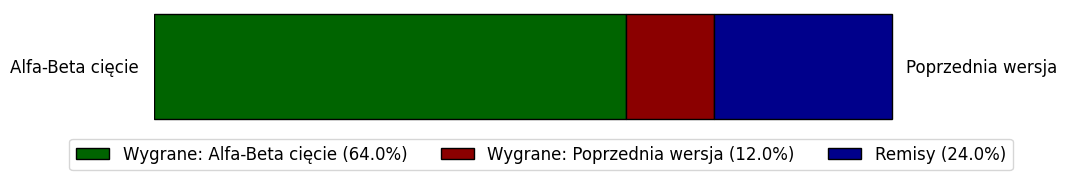
\includegraphics[width=1\textwidth]{rysunki/wyniki-alfa-beta}
                    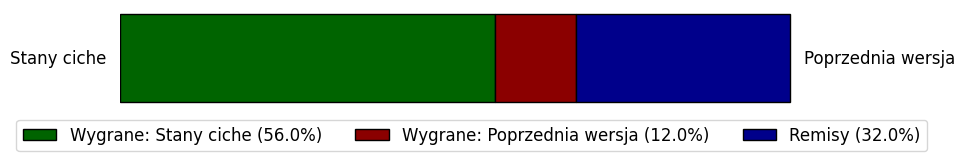
\includegraphics[width=1\textwidth]{rysunki/wyniki-stany-ciche}
                    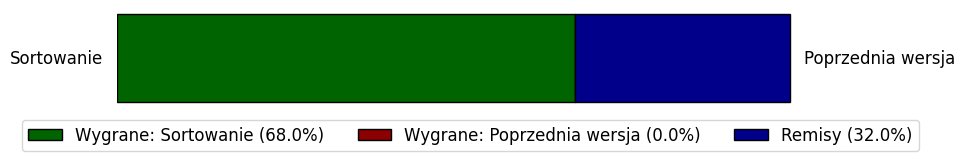
\includegraphics[width=1\textwidth]{rysunki/wyniki-sortowanie}
                    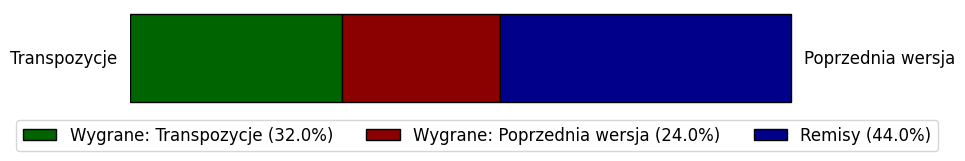
\includegraphics[width=1\textwidth]{rysunki/wyniki-transpozycje}
                }
            \end{block}

    \end{columns}

    \begin{block}{Lista zaimplementowanych ulepszeń algorytmów wyszukiwania}
        \centering {
            \small{Biblioteka otwarć, Alfa-Beta cięcie, Ewaluacja stanów cichych, Sortowanie ruchów, Tabela transpozycji, Okno estymacji.}
        }
    \end{block}



\end{frame}

\begin{frame}{Ulepszenia dla algorytmów wyszukiwania - II}
    \begin{flushright}
        \begin{table}[h!]
            \centering
            \resizebox{\textwidth}{!}{
                \begin{tabular}{|c|r|r|r|r|r|r|r|}
                    \hline
                    Start pos & Stockfish & Wersja podstawowa & Alfa-beta & Quiescence & Move ordering & Estimation & Transposition \\
                    \hline
                    1. & $20$ & $20$ & $20$ & $20$ & $20$ & $20$ & $20$ \\
                    2. & $400$ & $400$ & $186$ & $194$ & $214$ & $214$ & $214$ \\
                    3. & $8\,902$ & $8\,902$ & $2\,262$ & $2\,279$ & $2\,360$ & $2\,741$ & $2\,360$ \\
                    4. & $197\,281$ & $197\,281$ & $20\,596$ & $23\,119$ & $20\,428$ & $23\,597$ & $17\,481$ \\
                    5. & $4\,865\,609$ & $4\,865\,609$ & $223\,840$ & $225\,836$ & $173\,183$ & $199\,062$ & $123\,575$ \\
                    6. & $119\,060\,324$ & $119\,060\,324$ & $3\,349\,766$ & $1\,606\,833$ & $1\,019\,119$ & $1\,245\,427$ & $615\,267$ \\
                    7. & $3\,195\,901\,860$ & xxx & $20\,668\,442$ & $19\,449\,096$ & $7\,934\,005$ & $9\,078\,322$ & $3\,923\,917$ \\
                    8. & $84\,998\,978\,956$ & xxx & $275\,274\,306$ & $183\,000\,753$ & $57\,778\,837$ & $70\,097\,202$ & $23\,360\,242$ \\
                    \hline
                \end{tabular}
            }
            \label{tab:engine-comparison-1}
        \end{table}
        \begin{columns}
            \column{0.5\textwidth}
                \centering {
                    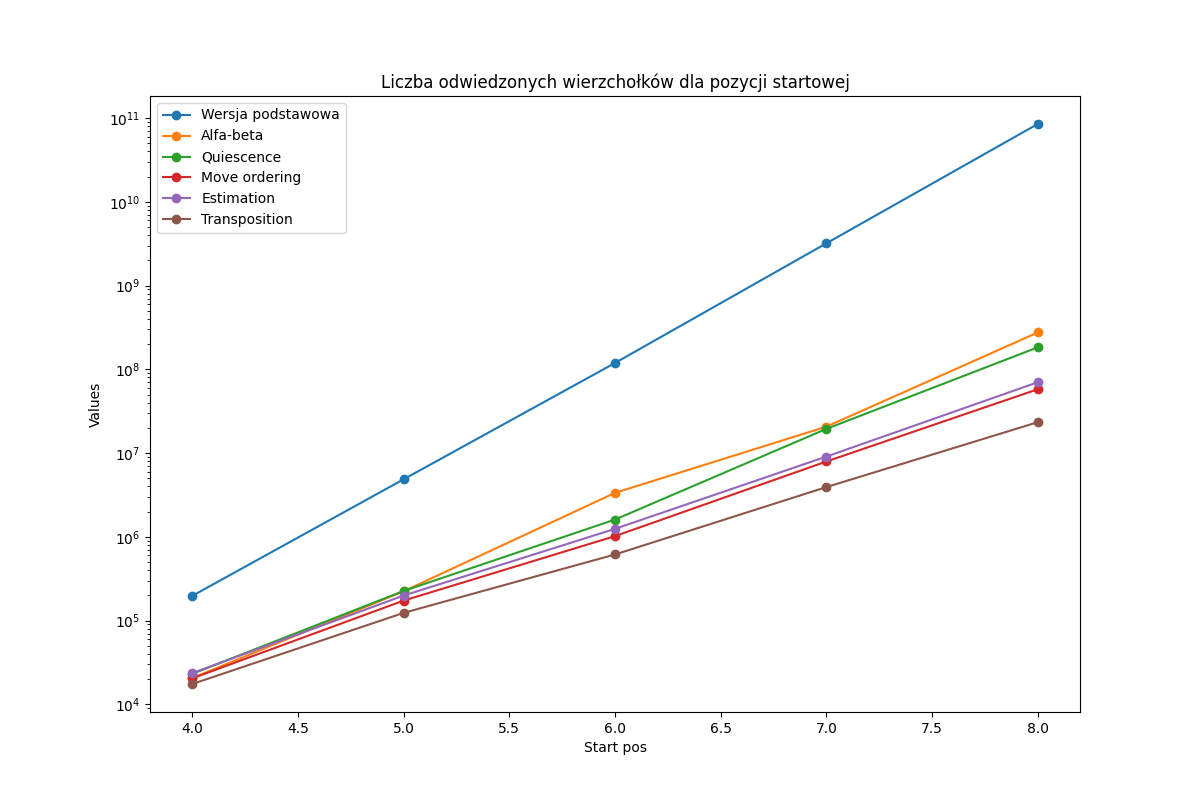
\includegraphics[width=1\textwidth]{rysunki/visited-chart}
                }
            \column{0.5\textwidth}
                \centering {
                    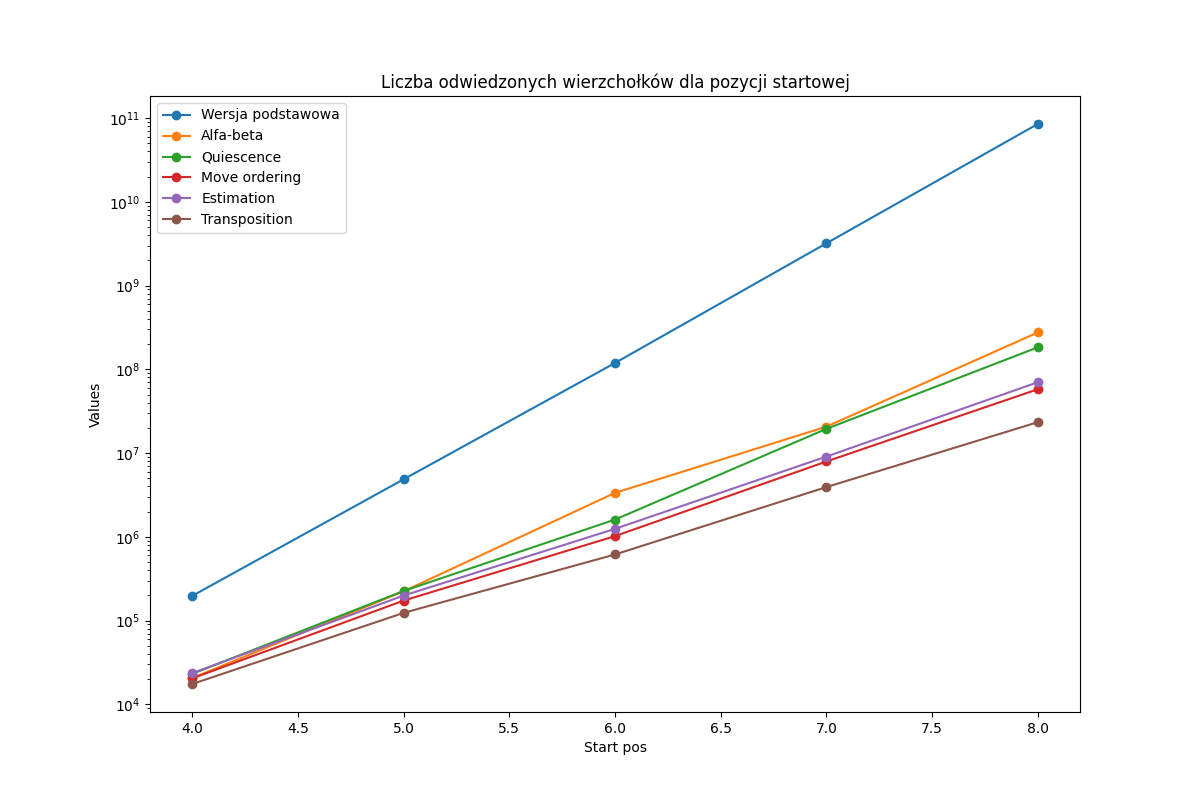
\includegraphics[width=1\textwidth]{rysunki/visited-chart}
                }
        \end{columns}
    \end{flushright}
\end{frame}

\begin{frame}{Ulepszenia dla oceny heurystycznej}

    \begin{columns}
        \column{0.5\textwidth}
            \begin{block}{Tablice figur}
                    \centering {
                        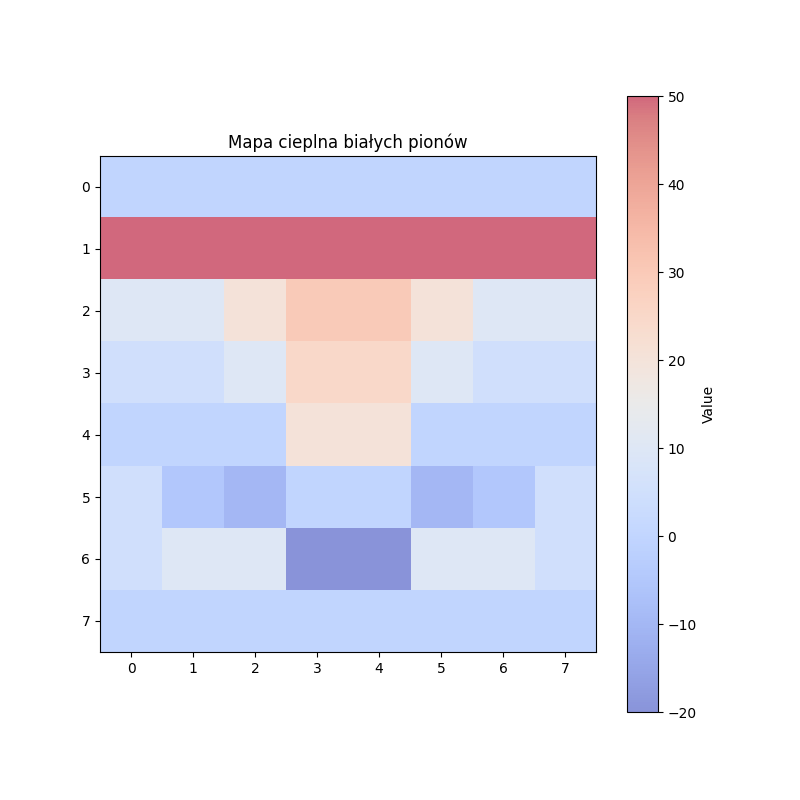
\includegraphics[width=0.6\linewidth]{rysunki/bialePiony}
                    }
            \end{block}
        \column{0.5\textwidth}
            \begin{block}{Wyniki rozgrywek}
                \centering {
                    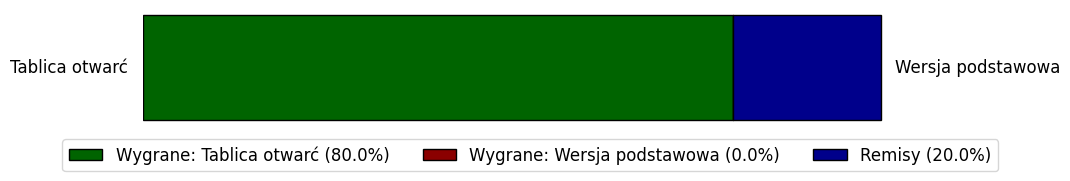
\includegraphics[width=1\linewidth]{rysunki/wyniki-tablica}
                    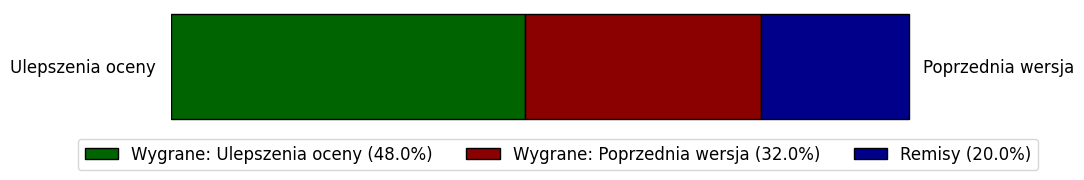
\includegraphics[width=1\linewidth]{rysunki/wyniki-full-eval}
                }
            \end{block}
    \end{columns}

    \begin{block}{Lista zaimplementowanych ulepszeń oceny heurystycznej}
        \centering {
            Tablice figur, Ochrona króla, Struktura pionów, Moment gry.
        }
    \end{block}
\end{frame}